\documentclass[11pt]{article}

\usepackage{physics}
\usepackage[top=1in, bottom=1in, left=1in, right=1in]{geometry}
\usepackage{hanging}
\usepackage{amsfonts, amsmath, amssymb}
\usepackage[none]{hyphenat}
\usepackage{fancyhdr}
\usepackage[nottoc, notlot, notlof]{tocbibind}
\usepackage{graphicx}
\graphicspath{{./images/}}
\usepackage{float}

\pagestyle{fancy}
\fancyhead{}
\fancyfoot{}
\fancyhead[L]{math seminars + physics club joint meeting 01/22/2020}
\fancyhead[R]{\thepage}
\renewcommand{\headrulewidth}{0pt}

\setlength{\parindent}{1cm}
\setlength{\parskip}{8pt}
\renewcommand{\baselinestretch}{1.15}

\newcommand{\ihat}{\boldsymbol{\hat{\textbf{\i}}}}
\newcommand{\jhat}{\boldsymbol{\hat{\textbf{\j}}}}
\newcommand{\dr}{\vec{r}~^{\prime}(t)}
\newcommand{\dx}{x^{\prime}(t)}
\newcommand{\dy}{y^{\prime}(t)}

\begin{document}

\setcounter{page}{1}

\begin{center}
The Fundamental Theorem of Line Integrals and Conservative Force Fields\\
Sai Sivakumar
\end{center}

In our introductory physics courses we know of several force fields. To name a few we have the electric, magnetic, and gravitational force fields. We can describe such fields more rigorously with vector calculus. But before that, we have to define certain operations and structures before we do anything.

What is a vector field?  - It is essentially a space in which each point in that space has a unique vector that corresponds to it. Graphically we depict these by drawing arrows (vectors) at reasonably spaced locations in space with its origin/tail at the point we are at and the tip pointing out in the direction of the vector with either its length or hue denoting magnitude. An example (incompletely drawn) field in two dimensions, $\mathbb{R}^2$, is as follows:

\begin{figure}[h]
\centering
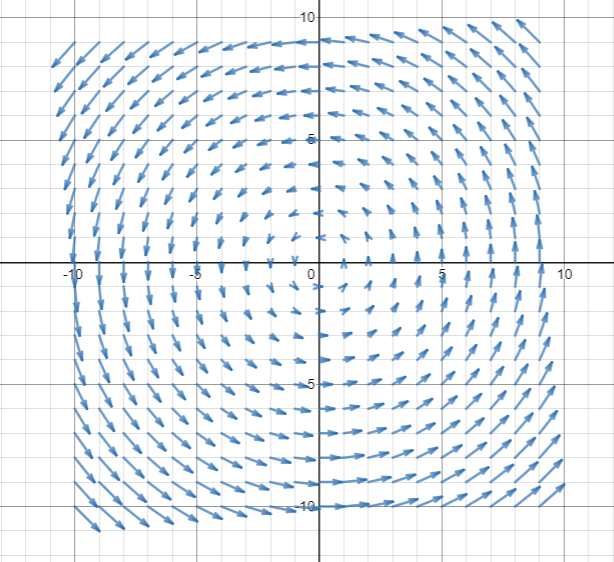
\includegraphics[scale=0.75]{examplefield}
\end{figure}

Mathematically a vector field $\vec{F}$ could take the following forms, but I prefer the engineering (the first) notation because I can write it in-line and it is standardized.

$$\vec{F} = P(x,y)\ihat + Q(x,y)\jhat ~=~ 
\begin{bmatrix}
P(x,y) \\
Q(x,y)
\end{bmatrix} ~=~ <P(x,y) , Q(x,y)>$$

The above notation simply states that the vector $\vec{F}$ produced at the location $(x,y)$ depends on the values $(x,y)$. The example field expressed mathematically is $\vec{F} = -y\ihat + x\jhat$.

For this demonstration, we focus on the electric, magnetic, and gravitational force fields because their behavior is dictated by the inverse square law, where the magnitude of force varies inversely with the square of the distance away from the source. But recall how each of these fields had a potential function associated with them - a common example is electric potential, or voltage, given by a charged particle. It varies inversely with the distance from the source, and in two dimensions it is described by a scalar function $\mathbb{R}^2 \to \mathbb{R}$. For a proton situated at the origin, the voltage plotted against location looks like the following:

\begin{figure}[h]
\centering
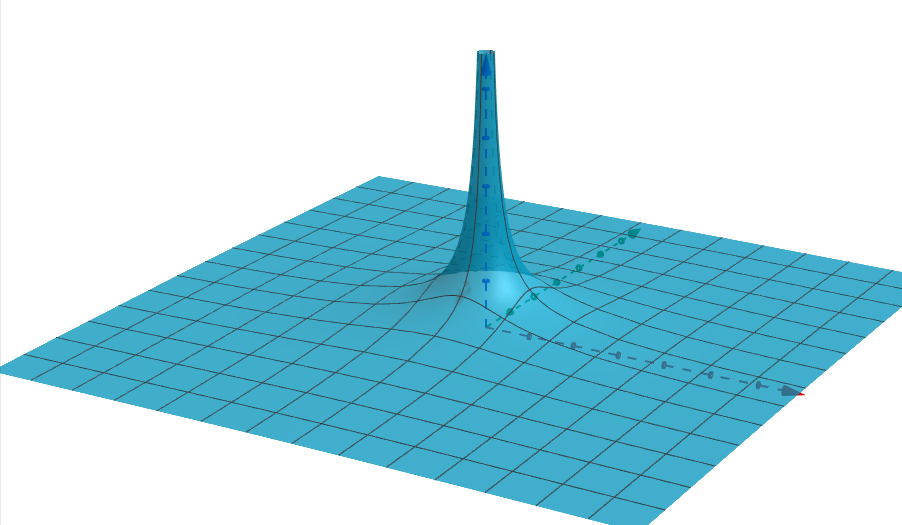
\includegraphics[scale=0.75]{examplevoltage}
\end{figure}

To get a two dimensional vector field, or the electric field,  from this voltage plot, we have to take the negative of the gradient of this scalar function. 

So what is the gradient? - it is an operator denoted by $\nabla$ that takes a scalar function and returns a vector field of one dimension less than that which the scalar function occupies. The components of the vector field are the partial derivatives of the scalar function taken in the axis matching the direction of the component. So for some scalar function of position $f(x,y)$ (or otherwise just called $f$), the gradient of it is as follows:

$$\nabla f(x,y) = \pdv{f}{x}\ihat + \pdv{f}{y}\jhat$$

The gradient is an analogue of the derivative in multiple variables that denotes locally the direction of greatest ascent. An example gradient of a paraboloid:

\begin{figure}[h]
\centering
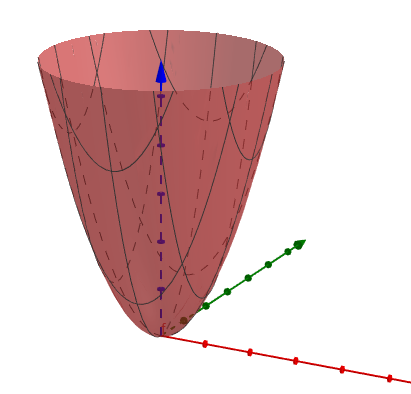
\includegraphics[scale=0.75]{paraboloidpart1}
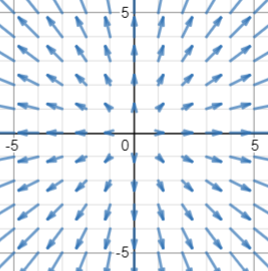
\includegraphics[scale=1]{paraboloidpart2}
\end{figure}

So for the voltage function, the negative of its gradient returns what is directions of steepest descent in potential energy for some positive charge placed anywhere. The magnitude of the field vectors of course is the magnitude of force it's going to experience just being there. Graphically the voltage function (like the example) and its electric field (scaled up) visually look like so:

\begin{figure}[h]
\centering
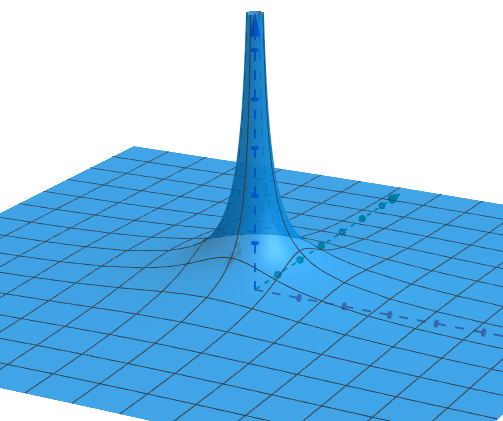
\includegraphics[scale=0.57]{voltagepart1}
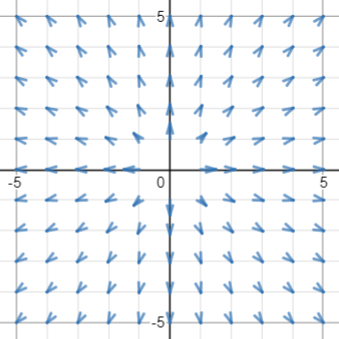
\includegraphics[scale=.75]{voltagepart2}
\end{figure}

Mathematically the electric field $\vec{E}$ is derived from voltage $V$ like so:

$$V = \frac{1}{r} = \frac{1}{(x^2+y^2)^{\frac{1}{2}}}$$
$$\nabla V = \pdv{V}{x}\ihat + \pdv{V}{y}\jhat = \left(\pdv{}{x} \frac{1}{(x^2+y^2)^{\frac{1}{2}}}\right) \ihat + \left(\pdv{}{y} \frac{1}{(x^2+y^2)^{\frac{1}{2}}}\right) \jhat = \frac{-x}{(x^2+y^2)^\frac{3}{2}} \ihat + \frac{-y}{(x^2+y^2)^\frac{3}{2}} \jhat$$

$$-\nabla V = \frac{x}{(x^2+y^2)^\frac{3}{2}} \ihat + \frac{y}{(x^2+y^2)^\frac{3}{2}} \jhat = \vec{E}$$

$$||\vec{E}|| = \sqrt{\left(\frac{x}{(x^2+y^2)^\frac{3}{2}}\right)^2 + \left(\frac{y}{(x^2+y^2)^\frac{3}{2}}\right)^2} = \frac{1}{(x^2+y^2)} = \frac{1}{r^2}$$

The elecric field, and other fields which follow the inverse square law like above, are all similar in this way. Then consider the following: Suppose we have a curve $C$ with direction defined by a set of position vectors given by $\vec{r}(t) = x(t)\ihat + y(t)\jhat$ (for $t \in [a,b]$, a time interval) embedded in the electric field, representing the path of a charged particle.

\begin{figure}[h]
\centering
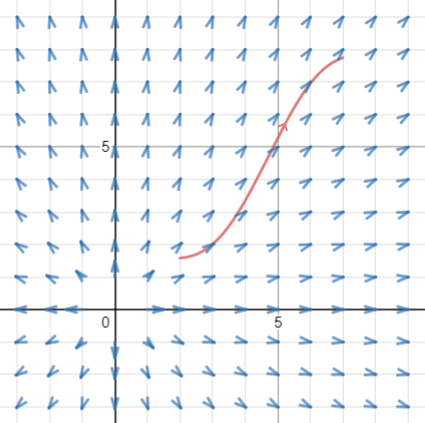
\includegraphics[scale=0.75]{curve}
\end{figure}

Desiring to compute the work done by the electrical force we compute the sum of the dot product of the force and the displacement at pretty much every spot on the curve in the right orientation. With the displacements approaching zero, the sum becomes the following integral in shorthand notation:

$$\int_C \vec{E}\cdot\dd{\vec{r}}$$

To actually evaluate this integral for example, we would have to replace $\dd{\vec{r}}$ with its differential form (using the velocity vector), replace $\vec{E}$ with $\vec{E}(x(t),y(t))$ to enumerate only those force vectors which lie on the curve, change the bounds to sum over $t$, simply take the dot product, and go through the algebra. Let us do that, then:

$$\int_C \vec{E}\cdot\dd{\vec{r}} \to \int_a^b \vec{E}(x(t),y(t))\cdot \dr \dd{t}$$
$$\int_a^b \vec{E}(x(t),y(t))\cdot \dr \dd{t} \to \int_a^b \left[\frac{x(t)}{(x(t)^2+y(t)^2)^\frac{3}{2}} \ihat + \frac{y(t)}{(x(t)^2+y(t)^2)^\frac{3}{2}} \jhat\right] \cdot \left[ \dx \ihat + \dy \jhat\right] \dd{t}$$

$$\int_a^b \left(\frac{x(t)}{(x(t)^2+y(t)^2)^\frac{3}{2}}\dx + \frac{y(t)}{(x(t)^2+y(t)^2)^\frac{3}{2}}\dy\right)\dd{t}$$

Here there is one more thing to introduce before we move further. The multivariable chain rule provides a way to determine the "total derivative" of a scalar function by parameterizing it into one variable. Its statement for an arbitrary function $f(x_1,x_2,x_3,...,x_n)$ is as follows: 

$$\dv{f}{t} = \sum_{k = 1}^n \pdv{f}{x_k (t)}x_k^{\prime}(t)$$

For this demonstration, let us parameterize the voltage function $V$ into $V(x(t),y(t))$ and take its derivative with respect to $t$.

$$\dv{V(t)}{t} = \frac{x(t)}{(x(t)^2+y(t)^2)^\frac{3}{2}}\dx + \frac{y(t)}{(x(t)^2+y(t)^2)^\frac{3}{2}}\dy$$

Conveniently this is found in the integrand and we can continue:

$$\int_a^b \left(\frac{x(t)}{(x(t)^2+y(t)^2)^\frac{3}{2}}\dx + \frac{y(t)}{(x(t)^2+y(t)^2)^\frac{3}{2}}\dy\right)\dd{t} \to \int_a^b V(t) \dd(t)$$

$$\int_a^b \dv{V(t)}{t} \dd(t) = V(b) - V(a)$$

Of course, to get the work from there you just multiply the result by the charge of the particle who took that path or whatever (really the specifics do not matter). What is important to realize is that the value of the integral depended only on the endpoints of the path, and this is true no matter how unusual the path is so long as it has derivatives that exist. This is why we call these fields conservative, because the value of the work the field does depends on the endpoints, and as a result if the charge takes a single circular path the work done is zero.

Some extra things involving more math that I will not be discussing involve a way to test if a field is conservative. To check if some arbitrary field is conservative, take the curl of the field, and if it equals zero everywhere then it is conservative. This is a result of Clairaut's theorem which states that  for a nice enough scalar function of two variables their mixed partial derivatives of the second order are equivalent. Try it yourself!

\begin{flushright}
Sai Sivakumar
\end{flushright}

\end{document}